\documentclass[notitlepage]{revtex4-1}
\usepackage{geometry}
\usepackage{graphicx}
\usepackage{times}
\usepackage{physics}   % for simple physics notation
\usepackage{bm}        % for math
\usepackage{amssymb}   % for math
\usepackage{amsmath}
\usepackage{subfigure}
\usepackage{color}
\usepackage{float}
\usepackage{enumitem}
\usepackage[export]{adjustbox}
\usepackage{comment}
\usepackage{listings}
\usepackage{CJK}
\usepackage{graphicx}
\newcommand{\hilight}[1]{\colorbox{red}{#1}}
%\usepackage{physics}
%\usepackage{enumerate}
%\usepackage{booktabs} % not allowed in Revtex4.1
\begin{document}
\begin{CJK}{UTF8}{bsmi}
\title{First Principle 2017-Fall  Homework 3 Solution}
%\input author_list.tex       % D0 authors (remove the first 3 lines
                             % of this file prior to submission, they
                             % contain a time stamp for the authorlist)
                             % (includes institutions and visitors)
\author{Kai-Hsin Wu (吳愷訢)}
\email{r05222003@ntu.edu.tw}
\affiliation{Department of Physics and Center of Theoretical Sciences, National Taiwan University, Taipei 10607, Taiwan}

%\date{\today}
\maketitle

\begin{enumerate}	
	\item The following shows the result of Al and Na:
		\begin{itemize}
			\item Al
			\begin{enumerate}[label=(\arabic*)]
				\item $a_0$ using volume optimization:
				\begin{equation*}
					a_0 = 4.05000 \hspace{0.2cm} 
				\end{equation*}
				\item Variation with different $a_0$:
					\begin{center}
					\begin{tabular}{ c c }
						$a_0$ & $E$ \\ 
						3.90 &-14.541085 \\
						3.95 &-14.665726\\
						4.00  &-14.735369\\
						4.05 &-14.757538\\
						4.10  &-14.738699\\
						4.15 &-14.684395\\
						4.20  &-14.599834 
					\end{tabular}
					\end{center}
				
				\item the following figure shows the energy ($E$ ) v.s. $V$ :
					\begin{figure}[!h]
						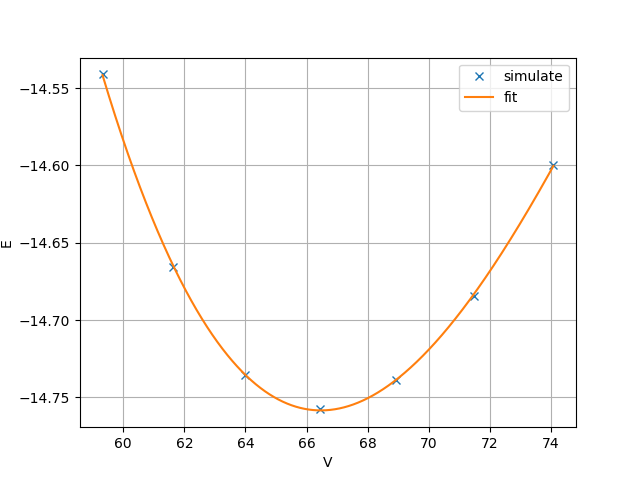
\includegraphics[width=8cm]{{Material/Al_E-V}.png}
						\caption{Al-fcc E-V}
						\label{fig:AlE-V}
					\end{figure}
					
					By using third order polyfit, and with the following formula, we can get the bulk-modulus $B$ and the minimum $a_0$:
					\begin{align*}
					B &= V\frac{\partial^2}{\partial V^2} E \\
					V &= a_0^3
					\end{align*}
					\begin{align*}
					a_{0} &= 4.050723 \hspace{0.2cm} \AA\\
					B  &= 74.608739 \hspace{0.2cm} GPar 
					\end{align*}
				
				\item  We start with HF energy density and seek for the minimum of $r_s$ :
				\begin{align*}
					e^{HF} = \frac{2.21}{r_s^2} - \frac{0.916}{r_s} 
				\end{align*}
				Where the unit of energy is $Ry$ and $r_s$ is in unit of bohr radius. The minimum is at :
				\begin{equation*}
					r_s = 2.553467 \hspace{0.2cm} \AA 
				\end{equation*} 
				using following relation by which we consider 1-free electron per unit-cell, we can estimate the lattice constant $a_0$ :
				\begin{align*}
					\frac{4\pi}{3}r_s^3 &= n^{-1} \\
					\frac{N_{free}}{a_0^3} &= n 
				\end{align*}
				
				\begin{align*}
					a_0 &= \left( \frac{4\pi}{3}\right)^{1/3} r_s \\
						&\approx 4.11616 \hspace{0.2cm} \AA \\
				\end{align*}

			\end{enumerate}
			\item Si
			
		\end{itemize}
\end{enumerate}




\bibliographystyle{apsrev4-1}
\bibliography{ref}
	
\end{CJK}
\end{document}

